\documentclass{article}
\usepackage{mathtools}
\usepackage[margin=0.95in]{geometry}
%\renewcommand{\familydefault}{\sfdefault}
\usepackage{amssymb}
\usepackage{cancel}
\usepackage{tikz-cd}
\usepackage{tikz}
\usepackage{caption}
\usepackage{pgfplots}
\usepackage{pgf}
\usepackage{centernot}
\usetikzlibrary{arrows,automata}
\usepackage{booktabs}
\usepackage{enumerate}
\usepackage{multirow}
%\usepackage{bbold}
\usepackage{changepage}
\pgfplotsset{compat = newest}
\usepackage{gensymb}
\usepackage[utf8]{inputenc}
\usepackage[english]{babel}
\usepackage{stmaryrd}
\usepackage{xcolor}
\usepackage{listings}
\definecolor{background}{RGB}{255,248,197}
\definecolor{gb}{RGB}{66, 133, 244}
\definecolor{gr}{RGB}{234, 67, 53}
\definecolor{gy}{RGB}{251, 188, 5}
\definecolor{gg}{RGB}{52, 168, 83}
\usepackage{color}
\usepackage{hyperref}
\hypersetup{colorlinks=true, linkcolor=black,
urlcolor=blue, linktoc=all}
\setcounter{MaxMatrixCols}{20}
\usepackage{witharrows}
\usepackage{graphicx}
\usepackage{float}
\usepackage{bm}
\usepackage{tabu}
\usepackage[many]{tcolorbox} %[enhanced,boxrule=0pt, frame hidden, sharp corners, borderline west={3pt}{-1.5pt}{black},breakable]
\usepackage{amsthm}
\usepackage{xfrac}
\usepackage{commath}
\usepackage{dirtytalk}
\usepackage{ytableau}
\newcommand{\inv}{^{-1}}
\newcommand{\qtq}[1]{\quad\text{#1}\quad}
\newcommand{\txt}[1]{\ \text{#1}\ }
\renewcommand{\ker}{\text{ker}}
\newcommand{\coker}{\text{coker}}
\newcommand{\Cor}{\text{Cor}_G(H)}
\newcommand{\ind}{\xrightarrow{d}}
\newcommand{\inp}{\xrightarrow{P}}
\newcommand{\almo}{\xrightarrow{\text{a.s}}}
\newcommand{\vecv}{\vec{v}}
\newcommand{\vecu}{\vec{u}}
\newcommand{\vecw}{\vec{w}}
\newcommand{\zmod}[1]{\Z/ #1 \Z}
\newcommand{\floor}[1]{\lfloor #1 \rfloor}
\newcommand{\lip}{\langle}
\newcommand{\rip}{\rangle}
\DeclareSymbolFont{symbolsC}{U}{txsyc}{m}{n}
\DeclareMathSymbol{\indep}{\mathrel}{symbolsC}{121}
\newcommand{\newpar}{\vspace{8pt}}
\renewcommand{\phi}{\varphi}
\newcommand{\ptwo}{p_\Lambda^{(2)}}
\newcommand{\pthree}{p_\Lambda^{(3)}}
\renewcommand{\epsilon}{\varepsilon}
\renewcommand{\theta}{\vartheta}
\DeclareMathOperator*{\argmax}{arg\,max}
\DeclareMathOperator{\deg}{deg}
\DeclareMathOperator*{\argmin}{arg\,min}
\DeclareMathOperator*{\limeaunf}{limea\"unf}
\newcommand{\Ree}{\text{Re}}
\newcommand{\Imm}{\text{Im}}
\newcommand{\iid}{\stackrel{\text{i.i.d}}{\sim}}
\newcommand{\rank}{\text{rank}}
\newcommand{\Span}{\text{span}}
\newcommand{\Int}{\text{Int}}
\newcommand{\Clos}{\text{Clos}}
\newcommand{\ideal}{\mathfrak{A}}
\newcommand{\idm}{\mathfrak{m}}
\newcommand{\idn}{\mathfrak{n}}
\newcommand{\idp}{\mathfrak{p}}
\newcommand{\idq}{\mathfrak{q}}
\newcommand{\limty}{\lim_{n\to\infty}}
\newcommand{\seq}[1]{(#1_n)_{n\geq1}}
\newcommand{\leteps}{\text{Let } \varepsilon > 0}
\renewcommand{\char}{\text{char}}
\newcommand{\mb}[1]{\bm{#1}}
\newcommand{\nil}{\text{nil}}
\newcommand{\code}[1]{\texttt{#1}}
\newcommand\bigzero{\makebox(0,0){\text{\huge0}}}
\renewcommand{\div}{\text{div}}
\newcommand{\R}{\mathbb{R}}
\newcommand{\N}{\mathbb{N}}
\newcommand{\C}{\mathbb{C}}
\renewcommand{\P}{\mathbb{P}}
\newcommand{\F}{\mathcal{F}}
\newcommand{\Z}{\mathbb{Z}}
\newcommand{\Q}{\mathbb{Q}}
\newcommand{\I}{\mathbb{I}}
\newcommand{\T}{\mathbb{T}}
\newcommand{\E}{\mathbb{E}}
\renewcommand{\S}{\mathbb{S}}
\newcommand{\zd}{\text{zd}}
\newcommand{\normal}{\vartriangleleft}
\newcommand{\Aut}{\text{Aut}}
\newcommand{\Inn}{\text{Inn}}
\newcommand{\ds}{\displaystyle}
\newcommand{\Vol}{\text{Vol}}
\newcommand{\sip}{(\ \ \mid\ \ )}
\newcommand{\intfin}{\int_{-\infty}^{\infty}}
\newcommand{\sumi}[1]{\sum_{i=1}^{#1}}
\newcommand{\ren}[1]{\mathbb{R}^{#1}}
\newcommand{\con}[1]{\mathbb{C}^{#1}}
\newcommand{\chisq}[1]{\chi^2_{#1}}
\newcommand{\orthcomp}{^{\perp}}
\newcommand{\im}{\text{im}}
\newenvironment{graytext}{\color{gray}}{\ignorespacesafterend}
\newcommand{\cov}{\text{cov}}
\newcommand{\var}{\text{var}}
\renewcommand{\l}{\left}
\renewcommand{\r}{\right}
\definecolor{codegreen}{rgb}{0,0.6,0}
\definecolor{codegray}{rgb}{0.5,0.5,0.5}
\definecolor{codepurple}{rgb}{0.58,0,0.82}
\definecolor{backcolour}{rgb}{0.95,0.95,0.92}
\mathtoolsset{showonlyrefs} 
\usepackage[utf8]{inputenc}
\setlength\parindent{0pt}

\lstdefinestyle{mystyle}{
    backgroundcolor=\color{backcolour},   
    commentstyle=\color{codegreen},
    keywordstyle=\color{magenta},
    numberstyle=\tiny\color{codegray},
    stringstyle=\color{codepurple},
    basicstyle=\ttfamily\footnotesize,
    breakatwhitespace=false,         
    breaklines=true,                 
    captionpos=b,                    
    keepspaces=true,                 
    numbers=left,                    
    numbersep=5pt,                  
    showspaces=false,                
    showstringspaces=false,
    showtabs=false,                  
    tabsize=2
}

\lstdefinestyle{python2}{
    language=Python,
    basicstyle=\ttfamily\small,
    keywordstyle=\color{blue},
    commentstyle=\color{gray},
    stringstyle=\color{red!60!black},
    showstringspaces=false,
    frame=single,
    numbers=left,
    numberstyle=\tiny\color{gray},
    tabsize=4,
    breaklines=true,
}

\title{\textbf{\textsf{Stat 175: Homework 3}}}
\author{\textsf{Matt Krasnow}}
\date{\textsf{Spring 2026}}

\begin{document}

\maketitle

Please submit your solutions to \href{https://www.gradescope.com/courses/1244242}{\underline{Gradescope}} by \textbf{Friday, February $\bm{20}^{\text{th}}$, 11:59pm}.\newpar

\begin{tcolorbox}[colback = gray!16, enhanced, boxrule=0pt, frame hidden, sharp corners, borderline west={3pt}{-1.5pt}{black!80},breakable]
\textbf{Exercise 1 (SBM Communities).} Let $G = (V, E)$ be a random graph on $n$ vertices from a Stochastic Block Model (SBM) with $k = 2$ communities. Each vertex $i$ belongs to community $z_i \in \{1, 2\}$ with equal probability: $\pi_1 = \pi_2 = \tfrac12$. Conditioned on the community labels $(z_i)_{i\in V}$, the edges are independent and satisfy
\begin{align}
    \P\l((i, j) \in E \mid z_i = a, z_j = b\r) = \begin{cases}
p, & a = b\\
q, & a \neq b.
    \end{cases}
\end{align}
for some $0 \leq p, q\leq1$. Thus $p$ is the within-community connection probability, and $q$ is the between-community connection probability. For two distinct vertices $i$ and $j$, define the number of common neighbors
\begin{align}
    C_{ij} = \abs{\{k \in V\setminus\{i, j\} : k \text{ is adjacent to both } i, j \}}.
\end{align}

\begin{enumerate}[$(a)$]
    \item Compute $\E[C_{ij} \mid z_i = z_j]$, the expected number of common neighbors of $i$ and $j$ when they are in the \textit{same} community.
    \item Compute $\E[C_{ij} \mid z_i \neq z_j]$, the expected number of common neighbors of $i$ and $j$ when they are in \textit{different} communities.
    \item Compare your two expressions. Which of the two expectations is larger (or are they equal)? Does your conclusion depend on whether $p>q$ or $p<q$?
    \item Based on your answers, propose a simple rule that attempts to decide whether a given pair $(i,j)$ belongs to the same community or to different communities.
\end{enumerate}
\end{tcolorbox}

\begin{tcolorbox}[colback=white, colframe=black!70, title=\textbf{Solution to Exercise 1}, breakable]
Let $V=\{1,\dots,n\}$ and fix distinct $i\neq j$. For each $k\in V\setminus\{i,j\}$ define the indicator
\[
I_k := \mathbf 1\{\text{$k$ adjacent to both $i$ and $j$}\}.
\]
Then
\[
C_{ij}=\sum_{k\neq i,j} I_k,\qquad \E[C_{ij}\mid \cdot]=\sum_{k\neq i,j}\E[I_k\mid \cdot].
\]
Conditioned on community labels, edges are independent, so
\[
\E[I_k\mid z_i,z_j,z_k]=\P((i,k)\in E\mid z_i,z_k)\cdot \P((j,k)\in E\mid z_j,z_k).
\]

\begin{enumerate}[(a)]
\item Assume $z_i=z_j$. Write $a:=z_i=z_j\in\{1,2\}$. For a given $k$,
\[
\E[I_k\mid z_i=z_j=a]=\E\Big[\P(i\sim k\mid a,z_k)\P(j\sim k\mid a,z_k)\,\Big|\,z_i=z_j=a\Big].
\]
Now $z_k=a$ with probability $1/2$ and $z_k\neq a$ with probability $1/2$.  
\begin{itemize}
\item If $z_k=a$, then $\P(i\sim k)=p$ and $\P(j\sim k)=p$, so the product is $p^2$.
\item If $z_k\neq a$, then $\P(i\sim k)=q$ and $\P(j\sim k)=q$, so the product is $q^2$.
\end{itemize}
Hence
\[
\E[I_k\mid z_i=z_j]=\frac12 p^2+\frac12 q^2.
\]
Summing over the $n-2$ possible $k$ gives
\[
\boxed{\ \E[C_{ij}\mid z_i=z_j]=(n-2)\cdot \frac{p^2+q^2}{2}\ }.
\]

\item Assume $z_i\neq z_j$. Without loss of generality take $z_i=1, z_j=2$. For a given $k$, we again average over $z_k$:
\begin{itemize}
\item If $z_k=1$ (probability $1/2$), then $i$ and $k$ are same-community so $\P(i\sim k)=p$, while $j$ and $k$ are different-community so $\P(j\sim k)=q$. Product: $pq$.
\item If $z_k=2$ (probability $1/2$), then $\P(i\sim k)=q$ and $\P(j\sim k)=p$. Product: $qp=pq$.
\end{itemize}
So in either case the product is $pq$, hence
\[
\E[I_k\mid z_i\neq z_j]=pq,
\]
and therefore
\[
\boxed{\ \E[C_{ij}\mid z_i\neq z_j]=(n-2)\,pq\ }.
\]

\item Compare:
\[
\E[C_{ij}\mid z_i=z_j]-\E[C_{ij}\mid z_i\neq z_j]
=(n-2)\left(\frac{p^2+q^2}{2}-pq\right)
=(n-2)\cdot \frac{(p-q)^2}{2}\ge 0.
\]
Thus
\[
\boxed{\ \E[C_{ij}\mid z_i=z_j]\ge \E[C_{ij}\mid z_i\neq z_j]\ \text{always, with equality iff } p=q.\ }
\]
So the ``same-community'' expectation is larger regardless of whether $p>q$ or $p<q$; it only depends on $p\neq q$.

\item A simple decision rule: for an observed pair $(i,j)$, compute $C_{ij}$. Since the expected number of common neighbors is larger when $i,j$ are in the same community (when $p\neq q$), a natural classifier is a threshold test:
\[
\text{declare } z_i=z_j \text{ if } C_{ij} \text{ is ``large,'' and } z_i\neq z_j \text{ otherwise.}
\]
One concrete choice is to compare $C_{ij}$ to the midpoint of the two conditional means:
\[
T := \frac12\Big(\E[C_{ij}\mid z_i=z_j]+\E[C_{ij}\mid z_i\neq z_j]\Big)
=(n-2)\left(\frac{p^2+q^2}{4}+\frac{pq}{2}\right).
\]
Then:
\[
\boxed{\ \text{Predict same community if } C_{ij}>T,\ \text{predict different if } C_{ij}<T\ (\text{ties arbitrary}).\ }
\]
(Any monotone threshold rule in $C_{ij}$ follows the same intuition.)
\end{enumerate}
\end{tcolorbox}

\vspace{12pt}

\begin{tcolorbox}[colback = gray!16, enhanced, boxrule=0pt, frame hidden, sharp corners, borderline west={3pt}{-1.5pt}{black!80},breakable]
\textbf{Exercise 2 (Contextualized SBM).} In the Contextualized Stochastic Block Model (CSBM), we observe both a graph $G$
and a set of node features $X$. Let $n$ be the number of nodes and $k= 2$ be the number of communities. Each node $i$ has a latent community $y_i \in\{+1,-1\}$ assigned uniformly
at random. Let $\bm v \sim N(0,\tfrac1d\mathbf I_d)$. We associate each node $i$ with a feature vector
\begin{align}
    X_i = \sqrt{\frac{1}{d}}y_i\frac{\bm v}{\|\bm v\|} + \sigma \mathbf Z_i,
\end{align}
where $\sigma > 0$ and $\mathbf Z_i \sim N(0, \tfrac1d\mathbf I_d)$. Suppose again that the within-community edge probability is $p_{11} = p_{-1, -1} = p$ and the between-community edge probability is $p_{1, -1} = q$. Let $n = 500$ and $d = 250$.
\begin{enumerate}[$(a)$]
    \item First, let us ignore the features $(X_i)$ for now, and focus only on the graph $G$. Recall the two main steps of the Spectral Clustering Algorithm mentioned in class:
    \begin{enumerate}[1.]
        \item Compute the eigenvector $e_2$ which corresponds to the second smallest eigenvalue $\lambda_2$ of the Laplacian matrix $L =  D-A$ (recall that we already know $\lambda_1 = 0$, and $e_1 = (1, \hdots, 1)$).
        \item Cluster the entries $(e_{2, i})_{i\leq n}$ using the $k$-means algorithm, and assign communities from this.
    \end{enumerate}
    Do the above algorithm for three different sets of values for $p$ and $q$:
    \begin{align}
        {p \choose q} = {0.8 \choose 0.6},\ \ {\frac{4\log^2(n)}{3n}\choose \frac{\log^2(n)}{n}},\ \ {\frac{4}{3n}\choose\frac1n}.
    \end{align}
    What do you observe?
    \item Imagine now that $\sigma = 0$, meaning $X_i = \sqrt{\frac{1}{d}}y_i\frac{\bm v}{\|\bm v\|}$. What is the top eigenvector of $\tfrac1dXX^\intercal$? If $\sigma$ is instead small but not exactly zero, what can we expect for the top eigenvector of $\tfrac1dXX^\intercal$?
    \item Implement the following spectral method: obtain the top eigenvector of $\tfrac1dXX^\intercal$, and call it $\hat v_1$. Run the $k$-means clustering algorithm on the entries of $\hat v_1$, and assign communities correspondingly. Do this for $\sigma = 0, 0.1, 0.5, 1.$ What do you observe?
    \item Now, for each vertex $i$, define the vector $B_i := (e_{2, i}, \hat v_{1, i})$. Run the $k$-means algorithm on $(B_i)_{i\leq n}$ and classify into communities again. What do you observe now?
\end{enumerate}
\end{tcolorbox}

\begin{tcolorbox}[colback=white, colframe=black!70, title=\textbf{Solution to Exercise 2}, breakable]

\begin{enumerate}[(a)]
\item Figure~\ref{fig:2a} shows the entries of $e_2$ (sorted by true label) for each $(p,q)$ regime.
\begin{itemize}
  \item \textbf{Dense regime} $(p,q)=(0.8,0.6)$: The two communities are perfectly separated by $e_2$; $k$-means recovers them exactly.
  \item \textbf{Logarithmic regime} $p=\tfrac{4\log^2 n}{3n},\ q=\tfrac{\log^2 n}{n}$: There is a clear sign flip in $e_2$ at the community boundary; clustering is again accurate.
  \item \textbf{Subcritical regime} $p=\tfrac{4}{3n},\ q=\tfrac{1}{n}$: The graph is very sparse and the eigenvector entries are essentially noise --- no community structure is visible and $k$-means fails.
\end{itemize}
\begin{figure}[H]
  \centering
  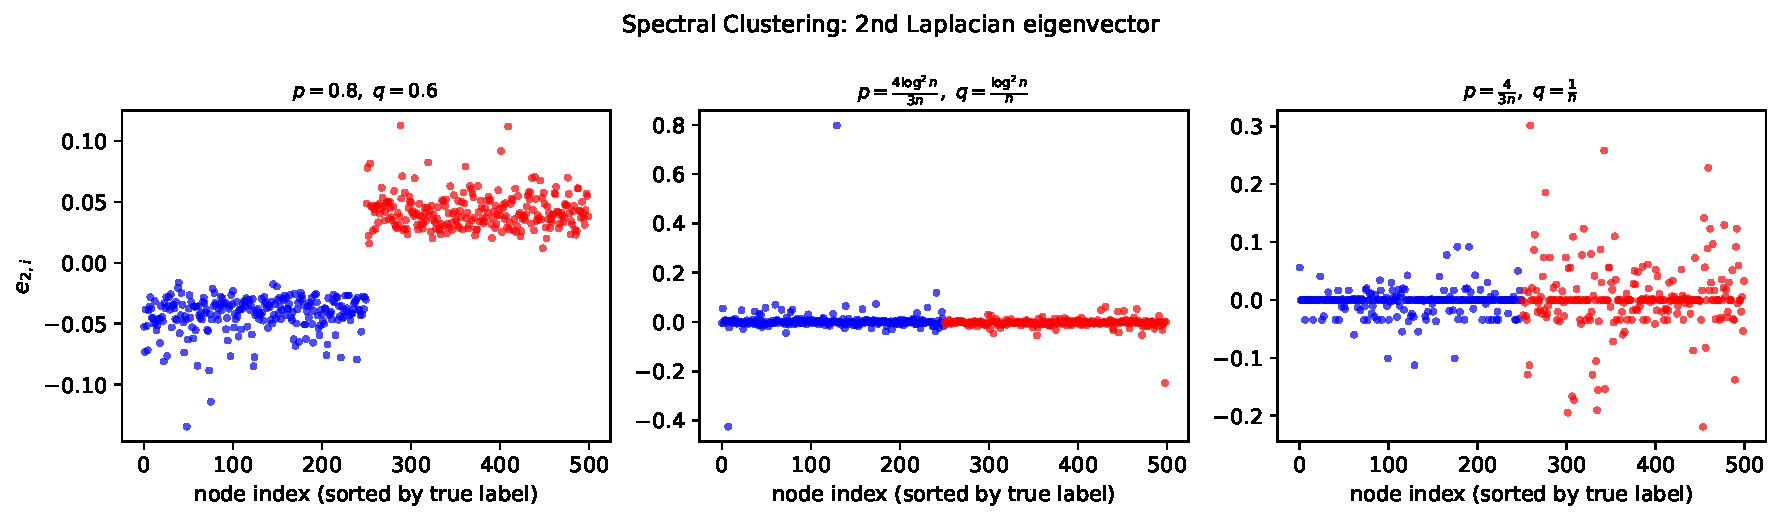
\includegraphics[width=\linewidth]{Figures/fig2a.pdf}
  \caption{Second eigenvector $e_2$ of $L=D-A$, entries coloured by true label ($+1$ red, $-1$ blue).}
  \label{fig:2a}
\end{figure}

\item \textbf{Top eigenvector of $\frac1d XX^\top$ for $\sigma=0$, and small $\sigma$.}

Let $y=(y_1,\dots,y_n)^\top\in\{\pm 1\}^n$ and define the unit direction $u:=\frac{\bm v}{\|\bm v\|}\in\R^d$ (well-defined a.s.). When $\sigma=0$, each feature vector is
\[
X_i=\sqrt{\frac1d}\,y_i\,u.
\]
Stacking rows gives an $n\times d$ matrix $X$ of the form
\[
X=\sqrt{\frac1d}\, y\, u^\top.
\]
Then
\[
XX^\top=\frac1d\, y\,u^\top u\, y^\top.
\]
Since $\|u\|=1$, we have $u^\top u=1$, so
\[
XX^\top=\frac1d\, y y^\top
\qquad\Rightarrow\qquad
\frac1d XX^\top=\frac1{d^2}\, y y^\top.
\]
This is a rank-one matrix. Its unique (up to sign) top eigenvector is proportional to $y$:
\[
y y^\top y = (y^\top y)\, y = n\, y,
\]
so the eigenvalue is $\frac{n}{d^2}$ and any unit-norm top eigenvector is
\[
\boxed{\ v_1 = \pm \frac{y}{\|y\|}=\pm \frac{y}{\sqrt n}\ }.
\]
Therefore, clustering the entries of $v_1$ perfectly recovers the two communities (up to label swap) when $\sigma=0$.

If $\sigma>0$ but small, write
\[
X=\sqrt{\frac1d}\, y u^\top + \sigma Z,
\]
where $Z$ has independent rows $Z_i\sim N(0,\tfrac1d I_d)$. Then
\[
\frac1d XX^\top
=
\underbrace{\frac1{d^2}\, y y^\top}_{\text{rank-1 signal}}
+
\underbrace{\frac{\sigma}{d}\Big(\sqrt{\frac1d} y u^\top Z^\top + \sqrt{\frac1d} Z u y^\top\Big)}_{\text{cross terms}}
+
\underbrace{\frac{\sigma^2}{d} ZZ^\top}_{\text{noise}}.
\]
Heuristically, this is a \emph{spiked} random matrix: a rank-one signal $y y^\top$ plus an approximately isotropic noise term. When $\sigma$ is small enough (signal-to-noise large enough), standard perturbation intuition (e.g.\ Davis--Kahan) says the top eigenvector remains \emph{close} to the signal direction $y$:
\[
\boxed{\ \text{For small }\sigma,\ \hat v_1 \text{ is strongly correlated with } y \text{ (close to }\pm y/\sqrt n\text{).}\ }
\]
As $\sigma$ increases, the top eigenvector becomes less aligned with $y$ and eventually can be dominated by the noise.

\item Figure~\ref{fig:2c} shows the entries of the top eigenvector $\hat v_1$ of $\tfrac1d XX^\top$ for each $\sigma$.
\begin{itemize}
  \item $\sigma=0$: $\hat v_1$ is exactly proportional to the label vector $y$; perfect clustering.
  \item $\sigma=0.1$: Still a clear two-block structure; near-perfect accuracy.
  \item $\sigma=0.5$: The signal is weaker but still visible; clustering succeeds with moderate error.
  \item $\sigma=1$: Noise dominates; the entries no longer separate into two groups and $k$-means largely fails.
\end{itemize}
\begin{figure}[H]
  \centering
  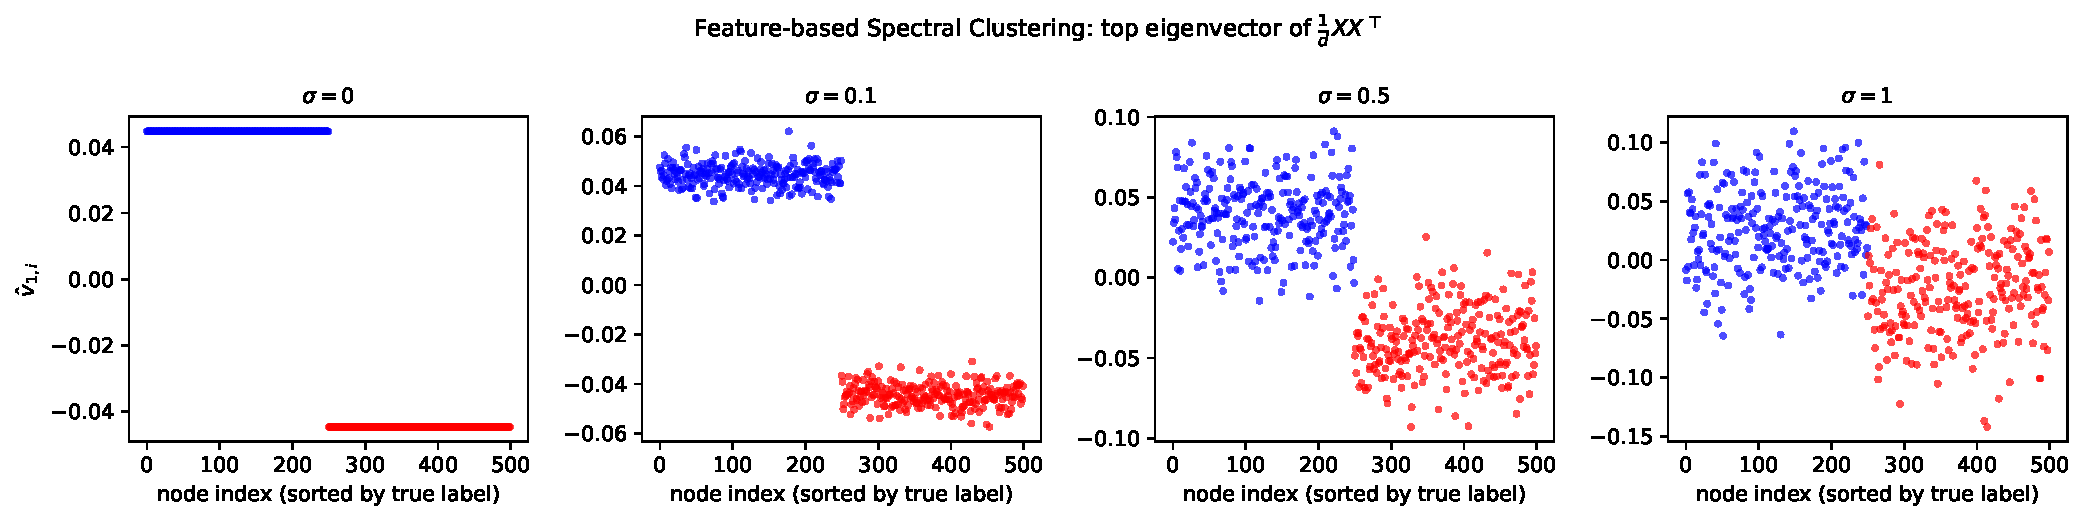
\includegraphics[width=\linewidth]{Figures/fig2c.pdf}
  \caption{Top eigenvector $\hat v_1$ of $\tfrac1d XX^\top$, entries coloured by true label, for $\sigma\in\{0,0.1,0.5,1\}$.}
  \label{fig:2c}
\end{figure}

\item Using the graph from the logarithmic $(p,q)$ regime (part (a)) and features with $\sigma=0.5$ (part (c)), we form $B_i=(e_{2,i},\hat v_{1,i})$ and run $k$-means on these 2-D vectors. Figure~\ref{fig:2d} shows the scatter plot of $B_i$ coloured by whether each node is correctly classified. Combining both sources of information yields better accuracy than either alone at $\sigma=0.5$: the graph eigenvector and the feature eigenvector each carry partial signal, and their union provides a cleaner separation boundary.
\begin{figure}[H]
  \centering
  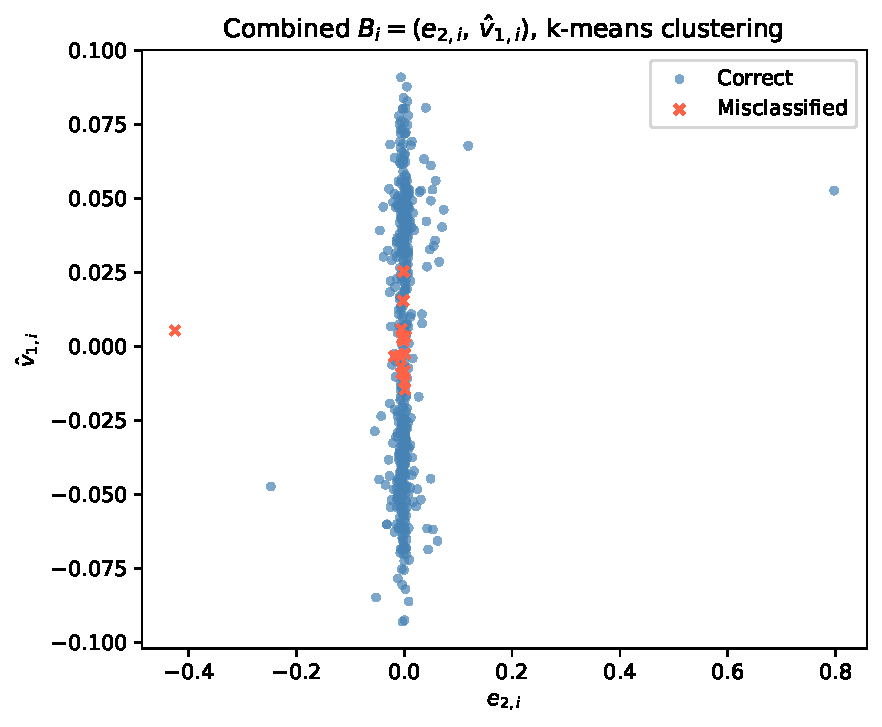
\includegraphics[width=0.55\linewidth]{Figures/fig2d.pdf}
  \caption{Scatter of $B_i=(e_{2,i},\hat v_{1,i})$; blue = correctly classified, red $\times$ = misclassified.}
  \label{fig:2d}
\end{figure}
\end{enumerate}
\end{tcolorbox}

\vspace{12pt}

\begin{tcolorbox}[colback = gray!16, enhanced, boxrule=0pt, frame hidden, sharp corners, borderline west={3pt}{-1.5pt}{black!80},breakable]
\textbf{Exercise 3 (Motifs in Erd\H{o}s--R\'enyi).} Consider the Erd\H{o}s--R\'enyi Random Graph $G(n,p)$ on vertices $\{1,\hdots, n\}$, where each edge exists independently with probability $p$. Let $H$ be a fixed simple graph (our motif) with vertex set $V(H)$ and edge set $E(H)$, and define 
\begin{align}
    v(H) := |V(H)|\quad\quad e(H) := |E(H)|\quad\quad d(H) := \frac{e(H)}{v(H)}.
\end{align}
Let $X$ be the number of (labelled) copies of $H$ inside our $G(n, p)$ graph.
\begin{enumerate}[$(a)$]
    \item Show that 
    \begin{align}
        \E[X] = \Theta\l(n^{v(H)}p^{e(H)}\r)\ \text{ as } \ n\to\infty,
    \end{align}
    where the implicit constants may depend on $H$, but not on $n$ or $p$. 
    \item Deduce that if 
    \begin{align}
        p \ll n^{-1/d(H)}\quad \l(\text{i.e., } p\cdot n^{1/d(H)} \to 0\r),
    \end{align}
    then we must have $\E[X] \to 0$ as $n\to\infty$.
    \item Conclude that, under this condition on $p$, the probability that $G(n,p)$ contains at
least one copy of $H$ also tends to 0 as $n\to\infty$. 
\end{enumerate}
\end{tcolorbox}

\begin{tcolorbox}[colback=white, colframe=black!70, title=\textbf{Solution to Exercise 3}, breakable]
Let $v:=v(H)=|V(H)|$ and $e:=e(H)=|E(H)|$. A \emph{labelled copy} of $H$ in $G(n,p)$ means an injective map
\[
\phi:V(H)\to [n]:=\{1,\dots,n\}
\]
such that for every edge $\{a,b\}\in E(H)$, the image $\{\phi(a),\phi(b)\}$ is an edge in $G(n,p)$. (Since $H$ is simple, this is the natural notion.)

For each injection $\phi$, define the indicator random variable
\[
I_\phi := \mathbf 1\{\text{$\phi$ is a graph embedding of $H$ into $G(n,p)$}\}.
\]
Then
\[
X=\sum_{\phi\ \text{injective}} I_\phi
\qquad\Rightarrow\qquad
\E[X]=\sum_{\phi\ \text{injective}} \E[I_\phi].
\]

\begin{enumerate}[(a)]
\item For a fixed injection $\phi$, the event $\{I_\phi=1\}$ requires that all $e$ edges of $H$ appear among the corresponding pairs in $G(n,p)$. In $G(n,p)$, edges appear independently with probability $p$, so
\[
\E[I_\phi]=\P(I_\phi=1)=p^{e}.
\]
It remains to count the number of injective maps $\phi:V(H)\to[n]$, which is the falling factorial
\[
(n)_v := n(n-1)\cdots (n-v+1).
\]
Therefore
\[
\E[X]=(n)_v\, p^e.
\]
Since $H$ is fixed (so $v$ is fixed) and $n\to\infty$, we have the standard asymptotic
\[
(n)_v = n^v\Big(1-\frac{1}{n}\Big)\Big(1-\frac{2}{n}\Big)\cdots \Big(1-\frac{v-1}{n}\Big)=\Theta(n^v),
\]
with implicit constants depending only on $v$ (hence only on $H$). Hence
\[
\boxed{\ \E[X]=\Theta\!\big(n^{v(H)}p^{e(H)}\big)\ \text{as } n\to\infty.\ }
\]

\item Recall $d(H)=e(H)/v(H)=e/v$. If $p\ll n^{-1/d(H)}$, then $p\, n^{1/d(H)}\to 0$, i.e.
\[
p\, n^{v/e}\to 0.
\]
Raise both sides to the power $e$ (note $e$ is fixed):
\[
p^e\, n^v \to 0.
\]
Using part (a), $\E[X]=\Theta(n^v p^e)$, so it follows that
\[
\boxed{\ \E[X]\to 0\ \text{as } n\to\infty.\ }
\]

\item Let $A$ be the event that $G(n,p)$ contains at least one copy of $H$. Then $A=\{X\ge 1\}$. By Markov's inequality,
\[
\P(X\ge 1)\le \E[X].
\]
Under the condition in (b), $\E[X]\to 0$, hence
\[
\boxed{\ \P\big(G(n,p)\text{ contains at least one copy of }H\big)=\P(X\ge 1)\to 0.\ }
\]
\end{enumerate}
\end{tcolorbox}

\vspace{12pt}

\end{document}
